Multi-objective optimization is characterized by the presence of multiple, possibly conflicting, objectives. This means that the optimal solution for any single objective doesn't necessarily correspond to the optimal solution for the other objectives. What we get instead is a set of solutions that are optimal in the sense that no other solution is better in all objectives. This set of solutions is called the Pareto front.

The state of the art in multi-objective optimization is the NSGA-II algorithm, which is a genetic algorithm that uses a non-dominated sorting approach to create fronts of solutions that are not dominated by any other solution. The algorithm then selects the best solutions from the fronts, ensuring that the population is diverse and that the Pareto front is well represented (maximimization of the crowding distance).

\subsection{Kursawe Function}
The Kursawe function is a simple test function for multi-objective optimization. It is defined as follows:
\begin{equation}
    \begin{cases}
        f_1(x) = \sum_{i=1}^{n-1} \left[ -10 \exp\left(-0.2\sqrt{x_i^2 + x_{i+1}^2}\right) \right] \\
        f_2(x) = \sum_{i=1}^{n} \left[ \left| x_i \right|^{0.8} + 5 \sin(x_i^3) \right]
    \end{cases}
\end{equation}

As a baseline, we use a simple Genetic Algorithm that combines the two objectives into a single one by taking a weighted sun of the two objectives in Table \ref{tab:kursawe_ga}.
\begin{table}[H]
    \centering
    \begin{tabular}{|c|c|c|c|c|}
        w1  & w2  & Fitness Mean       & Fitness Std.   & Best Fitness       \\ \hline
        1.0 & 0.0 & (-19.986, 0.085)   & (0.048, 0.041) & (-19.914, 0.018)   \\
        0.0 & 1.0 & (-12.913, -10.672) & (0.500, 0.362) & (-13.010, -10.748) \\
        0.5 & 0.5 & (-13.358, -10.562) & (0.056, 0.045) & (-13.375, -10.557) \\
        0.3 & 0.7 & (-13.154, -10.708) & (0.049, 0.024) & (-13.152, -10.717) \\
        0.7 & 0.3 & (-19.909, 0.095)   & (0.041, 0.021) & (-19.909, -0.0001) \\
    \end{tabular}
    \caption{Genetic Algorithm results for the Kursawe function with different weights}
    \label{tab:kursawe_ga}
\end{table}
We can see two different behavious depending on which one of the objectives is weighted more, but no solution is intrinsically better than the other.

Below we can compare the fitness of the final population of the Genetic Algorithm with the theoretical Pareto front of the Kursawe function.

\begin{figure}[H]
    \begin{subfigure}{0.5\textwidth}
        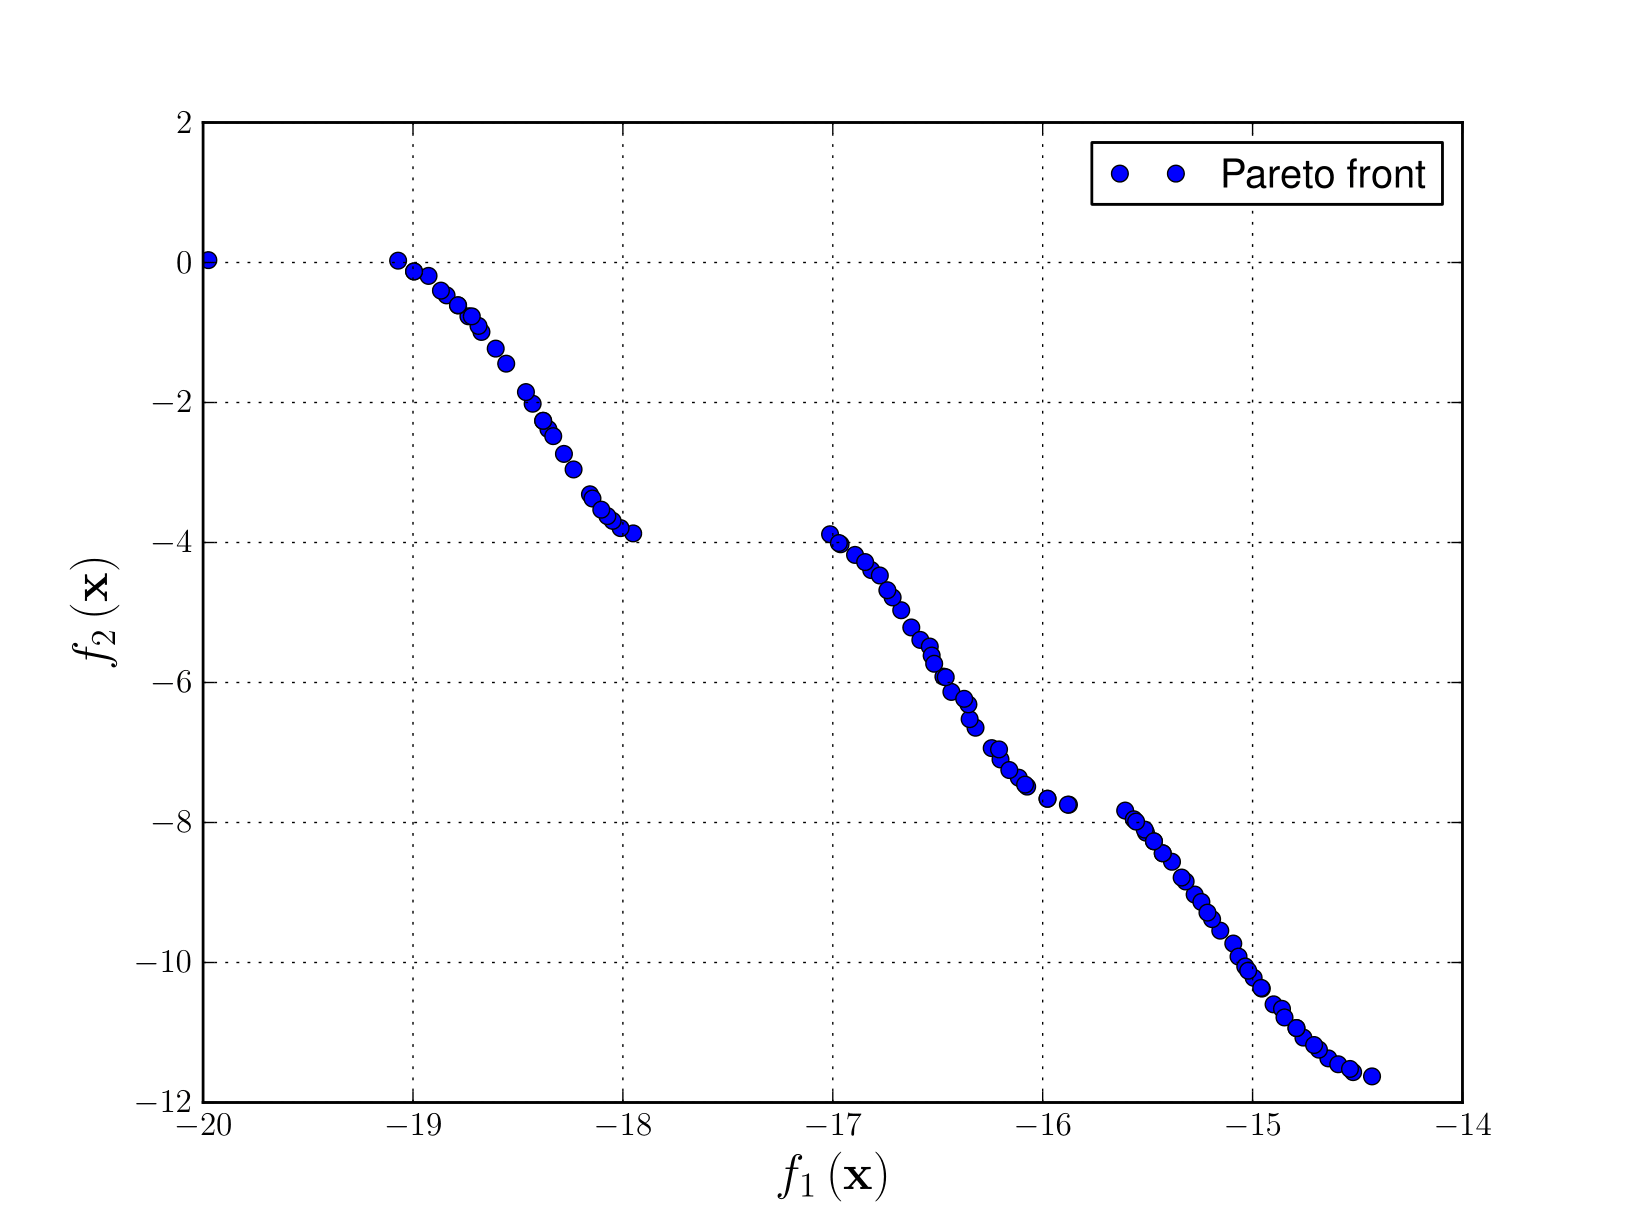
\includegraphics[width=\textwidth]{lab8/imgs/kursawe_theory.png}
        \caption{Theoretical Pareto front}
    \end{subfigure}
    \begin{subfigure}{0.5\textwidth}
        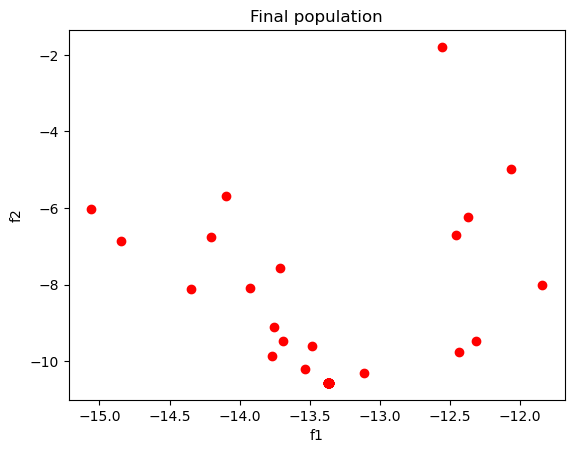
\includegraphics[width=\textwidth]{lab8/imgs/kursawe_ga.png}
        \caption{Genetic Algorithm (0.3, 0.7) weights}
    \end{subfigure}
    \label{fig:kursawe_ga}
    \caption{Comparison of the theoretical Pareto front and the final population of the Genetic Algorithm}
\end{figure}

We also solve the Kursawe function using the NSGA-II algorithm. The algorithm is able to find a set of solutions that are close to the theoretical Pareto front. The final population, sorted in the fronts created by the algorithm, is shown below.
\begin{figure}[H]
    \centering
    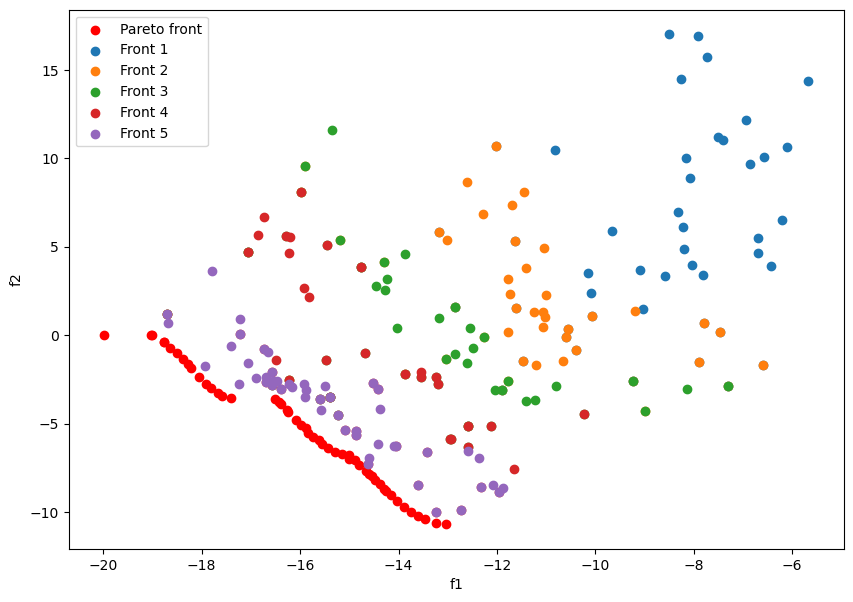
\includegraphics[width=\textwidth]{lab8/imgs/kursawe_nsga.png}
    \caption{NSGA-II final population}
    \label{fig:kursawe_nsga}
\end{figure}

\begin{table}[H]
    \centering
    \begin{tabular}{|c|c|c|}
        Objective & Best Fitness Mean & Best Fitness Std. \\ \hline
        f1        & -19.9022          & 0.0521            \\
        f2        & -10.5181          & 0.1668            \\
    \end{tabular}
    \caption{NSGA-II results for the Kursawe function}
    \label{tab:kursawe_nsga}
\end{table}
We can see how the simple genetic algorithm is able to find solutions that are close in one of the objectives to the NSGA-II results, but the final population doesn't resemble the Pareto front.

\subsection{Multiple-Disk Clutch Brake Optimization}
Real-world problem consisting of the optimization of five different parameters concerning the design of a multiple-disk clutch brake. The parameters are:
\begin{enumerate}
    \item $r_i \in [60,61,...,79,80]mm$ - inner radius of the disks
    \item $t_o \in [90,91,...,109,110]mm$ - outer radius of the disks
    \item $F \in [600,610,...,990,1000]N$ - force applied to the disks
    \item $t \in [1,1.5,2,2.5,3]mm$ - thickness of the disks
    \item $Z \in [2,3,4,5,6,7,8,9,10]$ - number of disks
\end{enumerate}
The two conflicting objectives are:
\begin{enumerate}
    \item minimization of the break system mass
    \item minimization of the stopping time
\end{enumerate}
We also consider an additional situation (constrained) where the fitness value of an individual is penalized every time the constraints on the range of the parameters are violated.
\begin{table}[H]
    \centering
    \begin{tabular}{|c|c|c|c|c|c|}
        Constrained & w1  & w2  & Fitness Mean    & Fitness Std.      & Best Fitness    \\ \hline
        False       & 1.0 & 0.0 & (0.187, 20.63)  & (8.32e-17, 3.249) & (0.187, 17.900) \\
        False       & 0.0 & 1.0 & (3.305, 3.378)  & (0.935, 0.055)    & (2.095, 3.317)  \\
        False       & 1.0 & 1.0 & (0.624, 3.730)  & (1.11e-16, 0.074) & (0.624, 3.730)  \\
        False       & 1.0 & 2.0 & (0.624, 3.791)  & (1.11e-16, 0.054) & (0.624, 3.731)  \\
        False       & 2.0 & 1.0 & (0.624, 3.788)  & (1.11e-16, 0.096) & (0.624, -3.731) \\ \hline

        True        & 1.0 & 0.0 & (0.187, 20.631) & (8.32e-17, 3.249) & (0.187, 17.900) \\
        True        & 0.0 & 1.0 & (3.305, 3.378)  & (0.935, 0.055)    & (2.095, 3.317)  \\
        True        & 1.0 & 1.0 & (0.624, 3.738)  & (1.11e-16, 0.074) & (0.624, 3.730)  \\
        True        & 1.0 & 2.0 & (0.624, 3.791)  & (1.11e-16, 0.054) & (0.624, 3.731)  \\
        True        & 2.0 & 1.0 & (0.624, 3.788)  & (1.11e-16, 0.096) & (0.624, -3.731) \\
    \end{tabular}
    \caption{Genetic Algorithm results for the Kursawe function with different weights}
    \label{tab:disk_ga}
\end{table}
We can see that the results for the constrained and uncostrained cases are basically the same, which means that the constraints are never violated. We can also observe that the first objective is much simpler to optimize given how low the standard deviation is compared to the second objective.

As for NSGA-II, we can see that the achieved Pareto front has slightly better results in the constrained case specifically in terms of crowding distance and optimization of the second objective. The final population divided into fronts for both scenarios is shown below.
\begin{figure}[H]
    \begin{subfigure}{0.5\textwidth}
        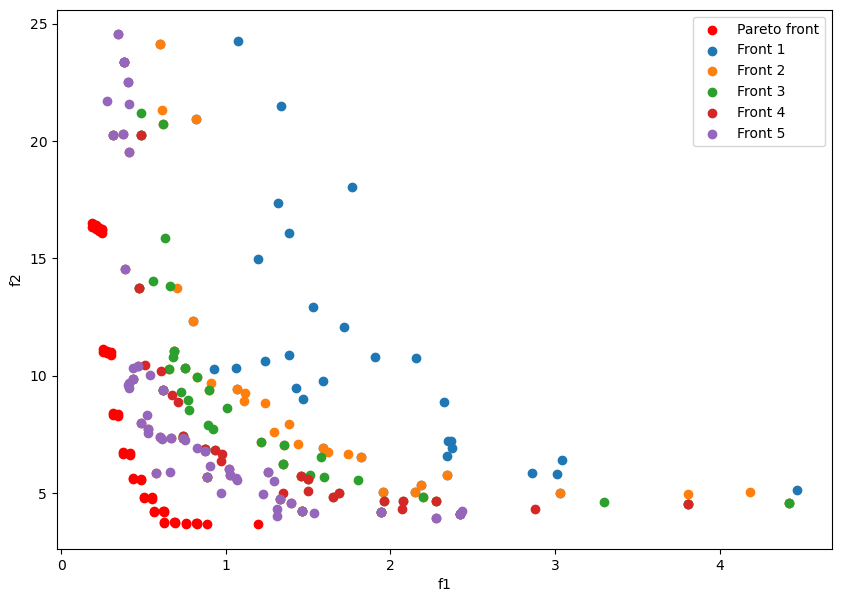
\includegraphics[width=\textwidth]{lab8/imgs/disk_nsga.png}
        \caption{NSGA-II final population}
    \end{subfigure}
    \begin{subfigure}{0.5\textwidth}
        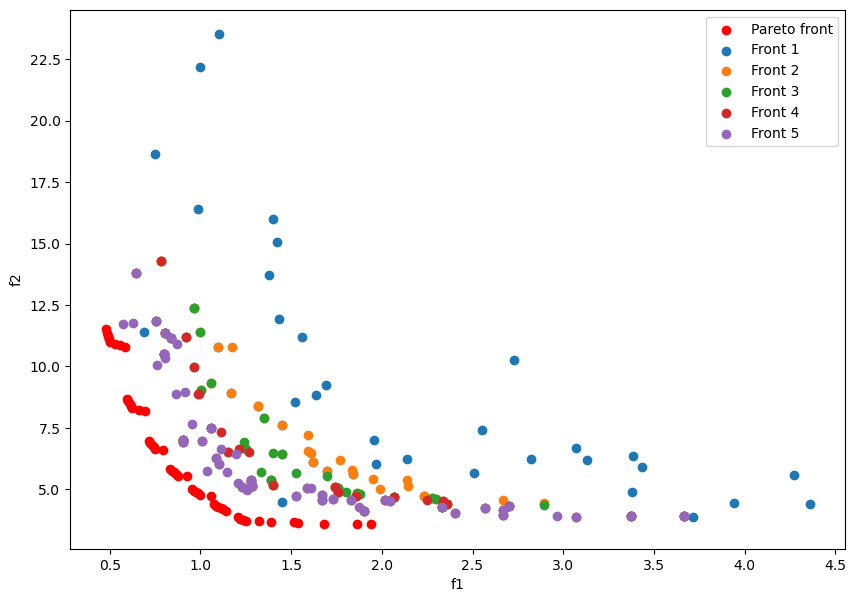
\includegraphics[width=\textwidth]{lab8/imgs/disk_constr_nsga.png}
        \caption{NSGA-II final population (constrained)}
    \end{subfigure}
\end{figure}

\begin{table}[H]
    \centering
    \begin{tabular}{|c|c|c|c|}
        \hline
        Constrained & Objective & Best Fitness Mean & Best Fitness Std. \\ \hline
        False       & f1        & -0.1874           & 8.32e-17          \\
        False       & f2        & 3.4276            & 0.1117            \\ \hline
        True        & f1        & 0.4900            & 0.0260            \\
        True        & f2        & 0.0853            & 0.0853            \\
    \end{tabular}
    \caption{NSGA-II results for the Kursawe function}
    \label{tab:disk_nsga}
\end{table}